\documentclass{beamer}

\usepackage[utf8]{inputenc}
\usepackage[T2A]{fontenc}
\usepackage[russian]{babel}

\usepackage{physics}
\usepackage{easyeqn}
\usepackage{amsmath}
% \usetheme{Madrid}

\usepackage[style=authortitle,backend=bibtex]{biblatex}
\addbibresource{refs.bib}

\usepackage[logo=sklogo]{beamerskoltech}

\DeclareMathOperator{\E}{\mathop{\mathbb{E}}}
\DeclareMathOperator*{\argmax}{arg\,max}
\DeclareMathOperator*{\argmin}{arg\,min}

\title{Bayesian Methods of Machine Learning.\\Project Presentation.\\Super-Samples from Kernel Herding}
\author{Georgii Novikov}
\date{October 2020}

\begin{document}
\maketitle

\begin{frame}{Super-Samples from Kernel Herding}
    \begin{block}{Weakly chaotic, non-linear dynamical system}
        \begin{EQA}[l] \label{nonkernel}
            x_{t + 1} = \argmax_{x \in \mathcal{X}} \langle w_t, \phi(x) \rangle \\
            w_{t + 1} = w_t + \E_{x \sim p} [\phi(x)] - \phi(x_{t + 1}) \\
            x_t \in \mathbb{R}^n, \phi : \mathbb{R}^{n} \rightarrow \mathbb{R}^m
        \end{EQA}
    \end{block}
    Under some conditions, it is a greedy minimization of
    \begin{EQA}[l] \label{nonkernel_error}
        \varepsilon_T^2 = \norm{\mu_p - \frac{1}{T}\sum_{t = 1}^T \phi(x_t)}^2, \text{where } \mu_p = \E_{x \sim p} \phi(x)
    \end{EQA}
\end{frame}

\begin{frame}{Theoretical Guarantees}
    \begin{block}{Theorem}
        $x_t$ in \eqref{nonkernel} is optimal on each step $\Rightarrow$ error in \eqref{nonkernel_error} decreases at a rate $\mathcal{O}(T^{-1})$.
    \end{block}
    \begin{block}{Advantage}
        \begin{enumerate}
            \item I.i.d samples have rate $\mathcal{O}(T^{-\frac{1}{2}})$
            \item MCMC converges even slower then $\mathcal{O}(T^{-\frac{1}{2}})$ (due to positive correlations)
        \end{enumerate}
    \end{block}
\end{frame}

\begin{frame}{Kernel Trick}
    We want to replace $\phi(x)$ with $k(x, x') = \langle \phi(x), \phi(x') \rangle$:
    \begin{enumerate}
        \item Define $w_0 = \mu := \E_{x \sim p} [\phi(x)]$
        \item
            \begin{EQA}[l]
                x_{t + 1} = \argmax_{x \in \mathcal{X}} \langle w_t, \phi(x) \rangle \\
                = \argmax_{x \in \mathcal{X}} \langle w_0 + T \E_{x' \sim p} [\phi(x')] - \sum_{t=1}^{T} \phi(x_t), \phi(x) \rangle \\
                = \argmax_{x \in \mathcal{X}} (T + 1) \E_{x' \sim p} k(x, x') - \sum_{t=1}^{T} k(x, x_t)
            \end{EQA}
    \end{enumerate}
\end{frame}

\begin{frame}{Interpretation}
    \begin{EQA}[l]
        \varepsilon_T^2 = \norm{\mu_p - \frac{1}{T}\sum_{t = 1}^T \phi(x_t)}^2_{\mathcal{H}} \\
        = \E_{x, x' \sim p} k(x, x') - \frac{2}{T}\sum_{i=1}^{T} \E_{x \sim p} k(x, x_t) + \frac{1}{T^2} \sum_{t, t'=1}^{T} k(x, x')
    \end{EQA}
    This is a measure between distribution $p$ and empirical distribution $\hat{p}_{T}(x) = \sum_{t=1}^{T} \delta(x, x_t)$. And we still have a rate of convergence $\mathcal{O}(T^{-1})$!
\end{frame}

\begin{frame}{Expiriment 0. Toy dataset}
    Mixture of 20 2D Gaussians: \\
    \begin{center}
        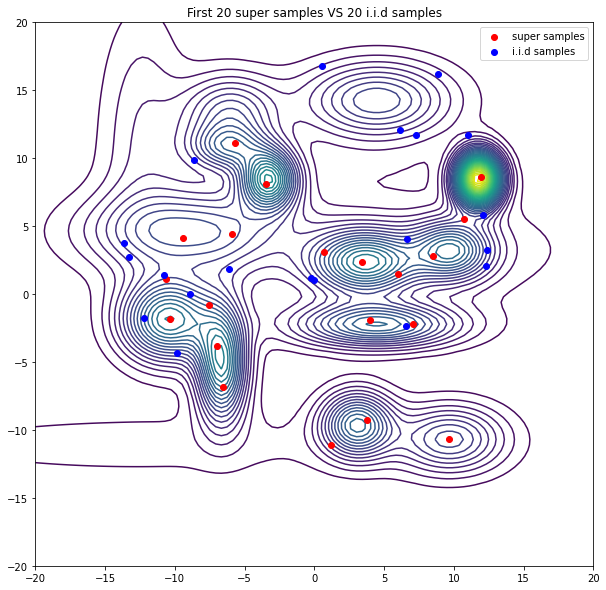
\includegraphics[width=.5\textwidth]{imgs/toy}
    \end{center}
\end{frame}

\begin{frame}{Expiriment 1. Empirical Matching}
    \begin{enumerate}
        \item $p(x) = $ mixture of 10 5D Gaussians
        \item $\mathcal{D} = 10^5 $ i.i.d samples
        \item Gaussian kernel $k$ (with $\sigma = 10$)
        \item Herding vs random samples on 4 functions of interest:
            \begin{enumerate}
                \item $\phi(x) = x^i, i \in {1, 2, 3}$
                \item $\phi(x) = sin(x)$
            \end{enumerate}
    \end{enumerate}
\end{frame}

\begin{frame}{Expiriment 1. Empirical Matching. Results}
    \begin{center}
        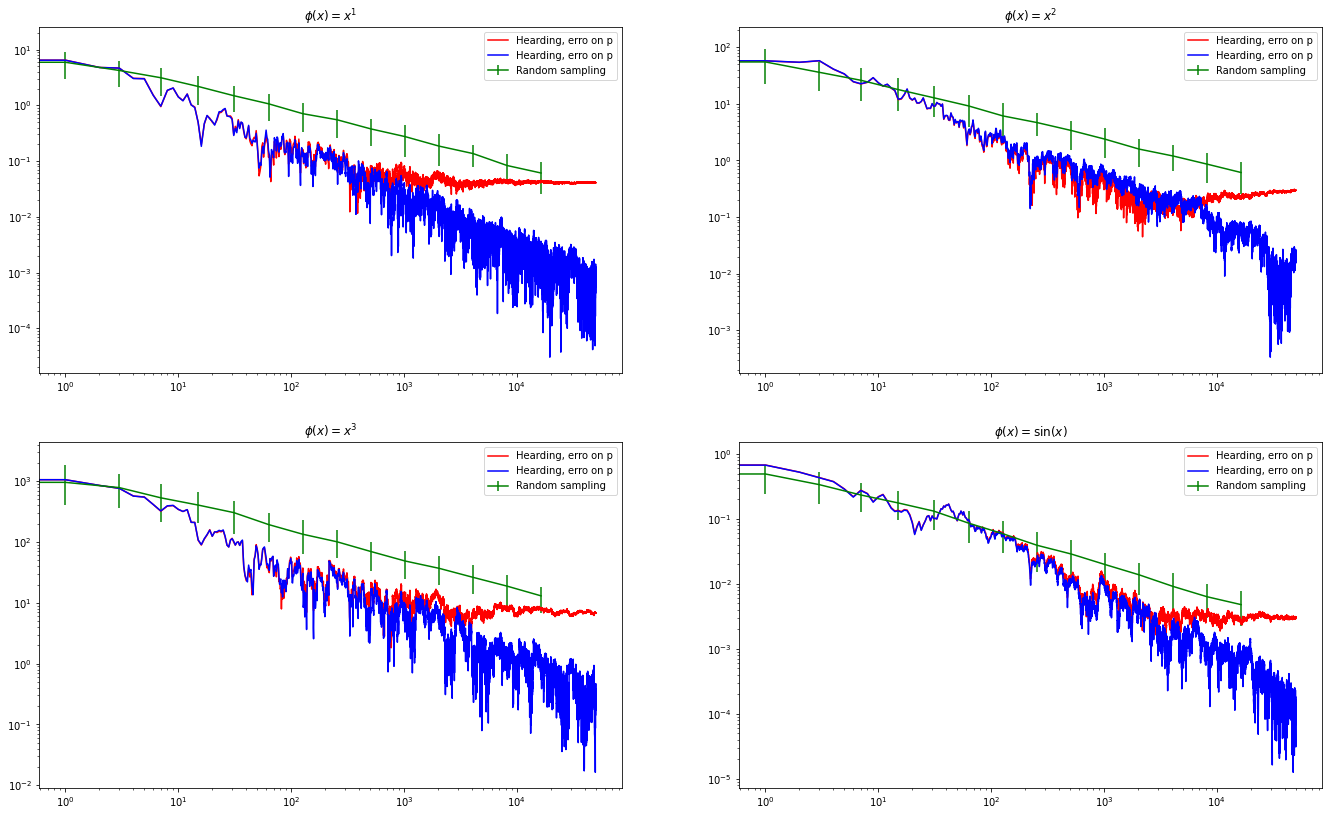
\includegraphics[width=\textwidth]{imgs/exp2}
    \end{center}
\end{frame}

\begin{frame}{Expiriment 2. Approximating the Bayesian Posterior}
    \begin{itemize}
        \item UCI spambase: 57 features. 4601 samples (3000 for train and 1601 for test).
        \item Whiten with PCA.
        \item Sample $10^7$ logistic regression parameters from the poster distribution with gaussian prior with Metropolis-Hasting and subsample to $10^5$ to reduce the autocorrelation.
        \item Whiten parameters with PCA.
        \item Herd super samples.
        \item Compare with metric
            \begin{EQA}[l]
                RMSE(S_T, D) = \frac{1}{N} \sum_{i=1}^{N} \left[ \frac{1}{T} \sum_{t=1}^{T} p(y_n | x_n, \theta_t) - \frac{1}{|D|} \sum_{d=1}^{|D|} p(y_n | x_n, \theta_d \right]
            \end{EQA}
    \end{itemize}
\end{frame}

\begin{frame}{Expiriment 2. Approximating the Bayesian Posterior. Result}
    \begin{center}
        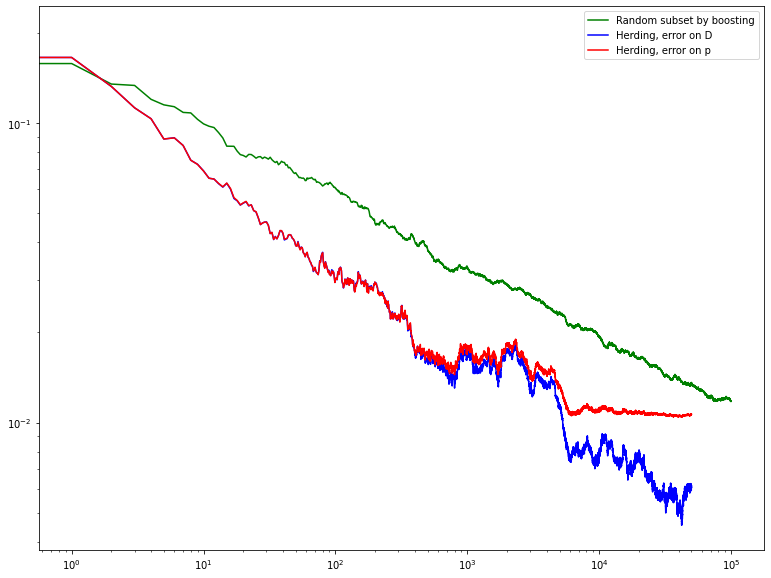
\includegraphics[width=.8\textwidth]{imgs/exp3}
    \end{center}
\end{frame}

\begin{frame}{Problems}
    Dependence on the parameters of Gaussian kernel is not clear.
    \begin{center}
        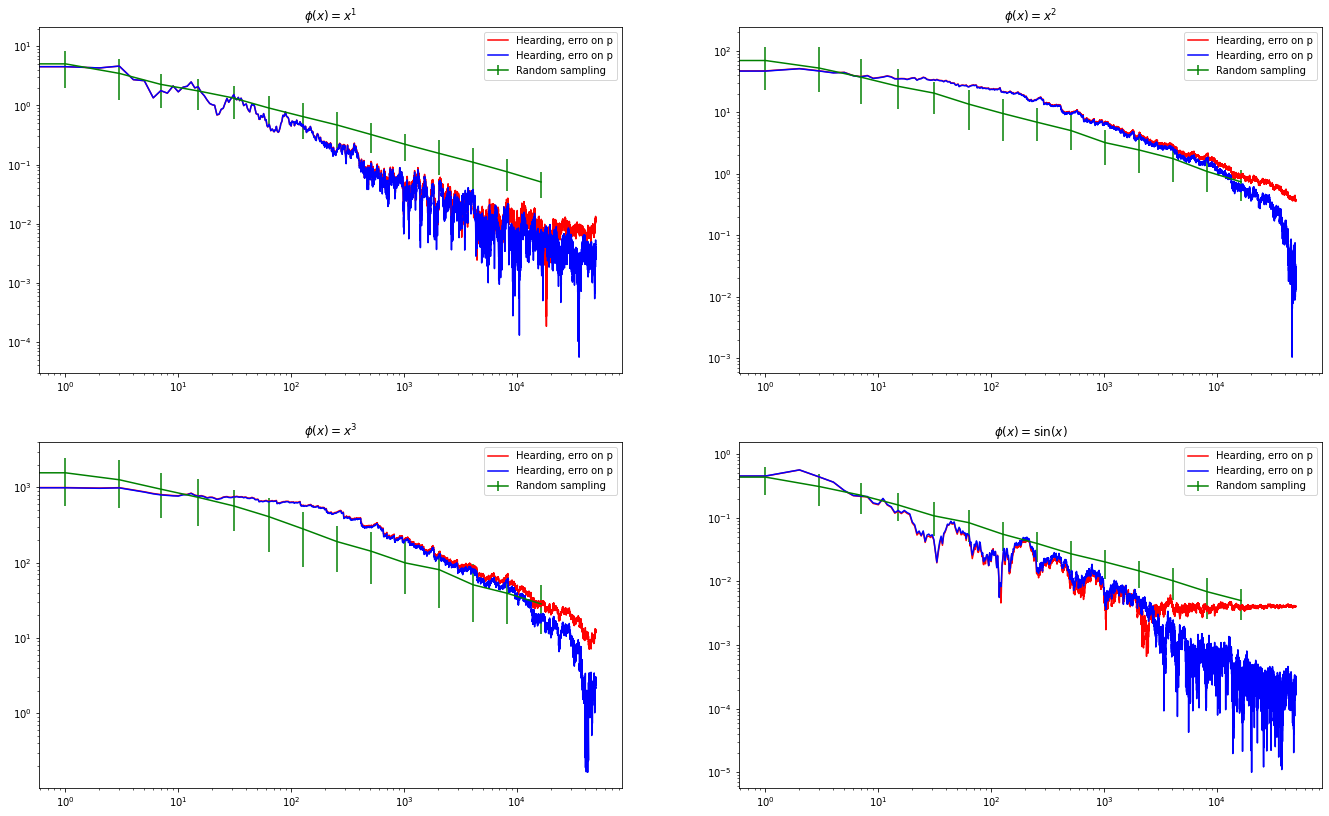
\includegraphics[width=.8\textwidth]{imgs/bad}
    \end{center}
\end{frame}



\end{document}
